\section{Results}
\subsection{I-V curves} \label{sec:results_iv}
Measures were conducted at temperatures between $(124 \pm 1)$ K and $(296\pm1)$ K. 
The acquired current-voltage curves and their fits from \autoref{eq:iv_curve} are depicted in \autoref{fig:iv-curves}.
The measures fit well with the thermionic emission model throughout the studied range of voltage, with currents of the order of the mA.
The barrier height $\Phi_b$ as a function of temperature, extrapolated from \autoref{eq:iv_curve}, is depicted in \autoref{fig:iv-barrier-height}.
$\Phi_b$ was observed to rise monotonically\hl{(linearly?)} with the temperature, ranging from $\sim 0.2 \pm ??$ eV at $(124 \pm 1)$ K to $\sim 0.5 \pm ??$ eV at $(296 \pm 1)$ K.

MODIFIED RICHARDSON PLOT \autoref{eq:richardson}.

\begin{figure}[htbp]
    \centering
    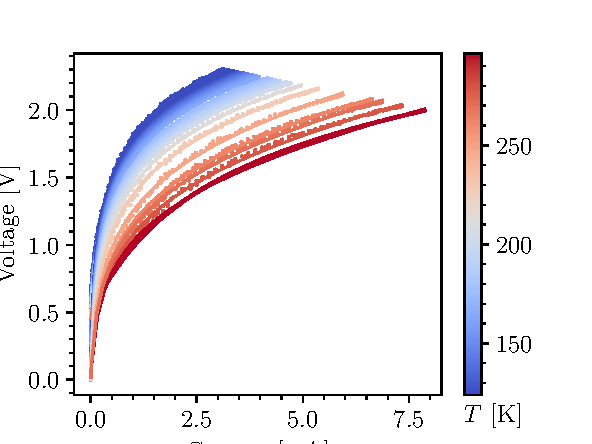
\includegraphics[scale=1]{figures/iv-curves.pdf}
    \caption{Current-Voltage curves measured over the metal-semiconductor junction at temperatures ranging from $??$ to $??$ K and related fits. \hl{TODO: marges figures}}
    \label{fig:iv-curves}
\end{figure}
\begin{figure}[htbp]
    \centering
    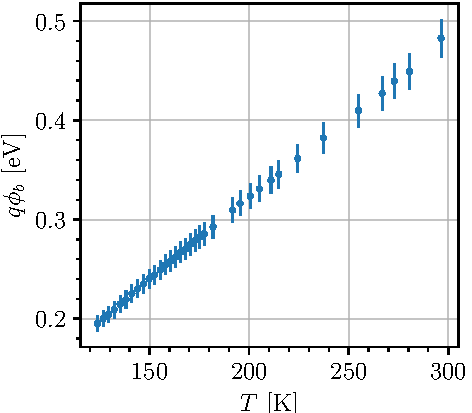
\includegraphics[scale=1]{figures/iv-schottky-potential-temperature.pdf}
    \caption{Schottky barrier height $\Phi_b$ as a function of temperature as obtained by I-V curves blabla. }
    \label{fig:iv-barrier-height}
\end{figure}
\begin{figure}[htbp]
    \centering
    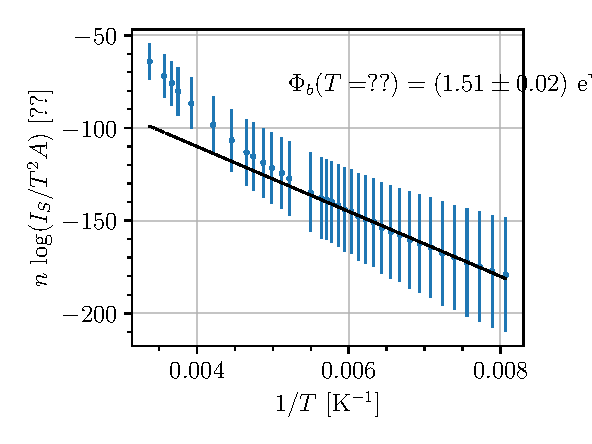
\includegraphics[scale=1]{figures/richardson.pdf}
    \caption{Modified Richardson plot.}
    \label{fig:richardson}
\end{figure}

\subsection{Internal photoemission} \label{sec:results_photoemission}
The photocurrent was measured between wavelengths $200$ nm and $1100$ nm.
\autoref{fig:photocurrent_curve} shows as an exemple the calibrated spectrum(\hl{square root of intensity of current vs $E$ of incoming photon}) acquired at $T = (100\pm3)$ K.
The linear portion between $\sim 1.3$ and $\sim 1.8$ eV was identified as the one related to photoemission and thus fit for fitting \hl{(ahah)} using \autoref{eq:fowler}.
The values of $\Phi_b$ obtained in each spectrum by finding the intercept with the $x$ axis are depicted in \autoref{fig:photoemission_phi}.
Contrary to what was found in  \autoref{sec:results_iv}, this method highlighted a barrier height decreasing with the temperature.



\begin{figure}[htbp]
    \centering
    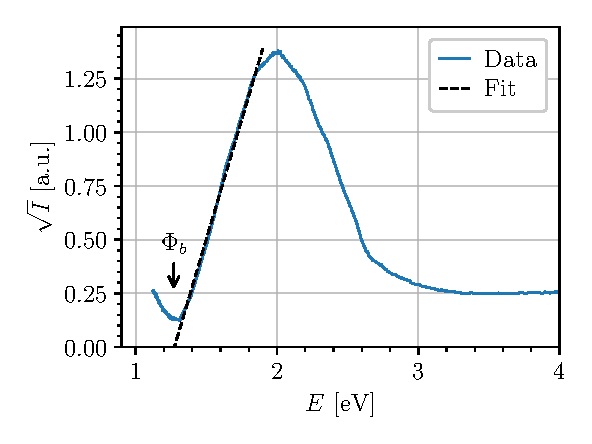
\includegraphics[scale=1]{figures/photocurrent_curve.pdf}
    \caption{Photocurrent measurement + fit}
    \label{fig:photocurrent_curve}
\end{figure}

\begin{figure}[htbp]
    \centering
    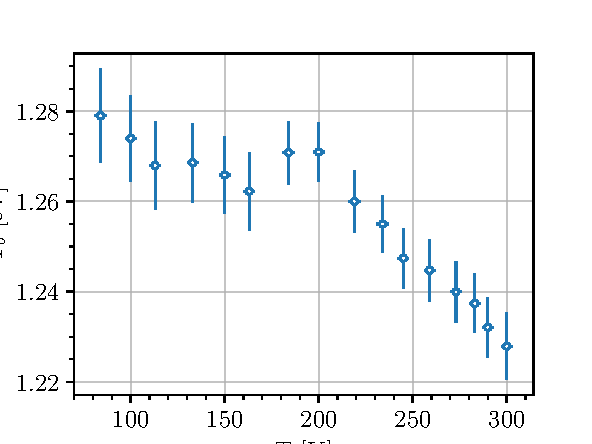
\includegraphics[scale=1]{figures/photoemission_phi.pdf}
    \caption{Schottky barrier height $\Phi_b$ as a function of temperature as obtained by photocurrent measurements}
    \label{fig:photoemission_phi}
\end{figure}


